\documentclass[11pt,utf8,notheorems,compress,t]{beamer}
\usepackage{etex}

\usepackage[english]{babel}

\usepackage{mathtools}
\usepackage{booktabs}
\usepackage{stmaryrd}
\usepackage{array}
\usepackage{ragged2e}
\usepackage{multicol}
\usepackage{tabto}
\usepackage{xstring}
\usepackage{ifthen}
\usepackage{soul}\setul{0.3ex}{}
\usepackage[all]{xy}
\xyoption{rotate}
\usepackage{tikz}
\usetikzlibrary{calc,shapes,shapes.callouts,shapes.arrows,patterns,fit,backgrounds,decorations.pathmorphing}
\hypersetup{colorlinks=true}
\usepackage{multimedia}
\newcommand{\video}[2]{\movie[width=#2,height=#2,autostart,loop,poster]{}{#1}}
\hypersetup{colorlinks=false}

\usepackage{pifont}
\newcommand{\cmark}{\ding{51}}
\newcommand{\xmark}{\ding{55}}
\DeclareSymbolFont{extraup}{U}{zavm}{m}{n}
\DeclareMathSymbol{\varheart}{\mathalpha}{extraup}{86}

\graphicspath{{images/}}

\usepackage[protrusion=true,expansion=true]{microtype}

\setlength\parskip{\medskipamount}
\setlength\parindent{0pt}

\title{Exploring the internal language of toposes}
\author{Ingo Blechschmidt}
\date{June 22nd, 2018 XXX}

\useinnertheme[shadow=true]{rounded}
\useoutertheme[subsection=false]{miniframes}
\setbeamerfont{block title}{size={}}

\useinnertheme{rectangles}

\usecolortheme{orchid}
\usecolortheme{seahorse}
\definecolor{mypurple}{RGB}{150,0,255}
\setbeamercolor{structure}{fg=mypurple}
\definecolor{myred}{RGB}{150,0,0}
\setbeamercolor*{title}{bg=myred,fg=white}
\setbeamercolor*{titlelike}{bg=myred,fg=white}
\setbeamercolor{frame}{bg=black}

\usefonttheme{serif}
\usepackage[T1]{fontenc}
\usepackage{libertine}

\newcommand{\A}{\mathcal{A}}
\newcommand{\B}{\mathcal{B}}
\renewcommand{\AA}{\mathbb{A}}
\renewcommand{\C}{\mathcal{C}}
\newcommand{\E}{\mathcal{E}}
\newcommand{\F}{\mathcal{F}}
\renewcommand{\G}{\mathcal{G}}
\newcommand{\GG}{\mathbb{G}}
\renewcommand{\O}{\mathcal{O}}
\newcommand{\K}{\mathcal{K}}
\newcommand{\NN}{\mathbb{N}}
\newcommand{\QQ}{\mathbb{Q}}
\newcommand{\RR}{\mathbb{R}}
\newcommand{\TT}{\mathbb{T}}
\newcommand{\PP}{\mathbb{P}}
\newcommand{\ZZ}{\mathbb{Z}}
\renewcommand{\P}{\mathcal{P}}
\newcommand{\aaa}{\mathfrak{a}}
\newcommand{\fff}{\mathfrak{f}}
\newcommand{\ppp}{\mathfrak{p}}
\newcommand{\mmm}{\mathfrak{m}}
\newcommand{\defeq}{\vcentcolon=}
\newcommand{\defeqv}{\vcentcolon\equiv}
\newcommand{\Sh}{\mathrm{Sh}}
\newcommand{\GL}{\mathrm{GL}}
\newcommand{\Zar}{\mathrm{Zar}}
\newcommand{\op}{\mathrm{op}}
\newcommand{\Set}{\mathrm{Set}}
\newcommand{\Eff}{\mathrm{Ef{}f}}
\newcommand{\Sch}{\mathrm{Sch}}
\newcommand{\Aff}{\mathrm{Aff}}
\newcommand{\LRS}{\mathrm{LRS}}
\newcommand{\Hom}{\mathrm{Hom}}
\newcommand{\Spec}{\mathrm{Spec}}
\newcommand{\lra}{\longrightarrow}
\newcommand{\RelSpec}{\operatorname{Spec}}
\renewcommand{\_}{\mathpunct{.}}
\newcommand{\?}{\,{:}\,}
\newcommand{\speak}[1]{\ulcorner\text{\textnormal{#1}}\urcorner}
\newcommand{\ull}[1]{\underline{#1}}
\newcommand{\affl}{\ensuremath{{\ull{\AA}^1}}}
\newcommand{\Ll}{\text{iff}}
\newcommand{\inv}{inv.\@}
\newcommand{\seq}{\vdash_{\!\!\!\vec x}}

\setbeamertemplate{blocks}[rounded][shadow=false]

% Adapted from https://latex.org/forum/viewtopic.php?t=2251 (Stefan Kottwitz)
\newenvironment<>{hilblock}{
  \begin{center}
    \begin{minipage}{9.05cm}
      \setlength{\textwidth}{9.05cm}
      \begin{actionenv}#1
        \def\insertblocktitle{}
        \par
        \usebeamertemplate{block begin}}{
        \par
        \usebeamertemplate{block end}
      \end{actionenv}
    \end{minipage}
  \end{center}}

\newcommand{\bignumber}[1]{
  \renewcommand{\insertenumlabel}{#1}\scalebox{1.5}{\usebeamertemplate{enumerate item}}
}
\newcommand{\bigheart}[1]{\scalebox{1.5}{\hil{$\varheart$}}}

\newenvironment{changemargin}[2]{%
  \begin{list}{}{%
    \setlength{\topsep}{0pt}%
    \setlength{\leftmargin}{#1}%
    \setlength{\rightmargin}{#2}%
    \setlength{\listparindent}{\parindent}%
    \setlength{\itemindent}{\parindent}%
    \setlength{\parsep}{\parskip}%
  }%
  \item[]}{\end{list}}

\newcommand{\hcancel}[5]{%
  \tikz[baseline=(tocancel.base)]{
    \node[inner sep=0pt,outer sep=0pt] (tocancel) {#1};
    \draw[red, line width=0.4mm] ($(tocancel.south west)+(#2,#3)$) -- ($(tocancel.north east)+(#4,#5)$);
  }%
}

\tikzset{
  invisible/.style={opacity=0,text opacity=0},
  visible on/.style={alt={#1{}{invisible}}},
  alt/.code args={<#1>#2#3}{%
    \alt<#1>{\pgfkeysalso{#2}}{\pgfkeysalso{#3}}}
}

\newcommand{\pointthis}[3]{%
  \tikz[remember picture,baseline]{
    \node[anchor=base,inner sep=0,outer sep=0] (#2) {#2};
    \node[visible on=#1,overlay,rectangle callout,rounded corners,callout relative pointer={(0.3cm,0.5cm)},fill=blue!20] at ($(#2.north)+(-0.1cm,-1.1cm)$) {#3};
  }%
}

% Adapted from https://latex.org/forum/viewtopic.php?t=2251 (Stefan Kottwitz)
\newenvironment<>{varblock}[2]{
  \begin{center}
    \begin{minipage}{#1}
      %\setlength{\textwidth}{#1}
      \begin{actionenv}#3
  \def\insertblocktitle{\centering #2}
  \par
  \usebeamertemplate{block begin}}{
        \par
        \usebeamertemplate{block end}
      \end{actionenv}
    \end{minipage}
  \end{center}}

\setbeamertemplate{frametitle}{%
  \vskip0.7em%
  \leavevmode%
  \begin{beamercolorbox}[dp=1ex,center]{}%
      \usebeamercolor[fg]{item}{\textbf{{\Large \insertframetitle}}}
  \end{beamercolorbox}%
}

\setbeamertemplate{navigation symbols}{}

\newcounter{framenumberpreappendix}
\newcommand{\backupstart}{
  \setcounter{framenumberpreappendix}{\value{framenumber}}
}
\newcommand{\backupend}{
  \addtocounter{framenumberpreappendix}{-\value{framenumber}}
  \addtocounter{framenumber}{\value{framenumberpreappendix}} 
}

\setbeamertemplate{headline}{%
  \begin{beamercolorbox}[wd=\paperwidth,ht=2.25ex]{}%
    \insertnavigation{\paperwidth}%
  \end{beamercolorbox}%
  \vskip0pt%
}

\setbeamertemplate{footline}{%
  \begin{beamercolorbox}[wd=\paperwidth,ht=2.25ex,dp=1ex,right,rightskip=1mm,leftskip=1mm]{}%
    % \inserttitle
    \hfill
    \insertframenumber\,/\,\inserttotalframenumber
  \end{beamercolorbox}%
  \vskip0pt%
}


\newcommand{\hil}[1]{{\usebeamercolor[fg]{item}{\textbf{#1}}}}

\newcommand{\bad}[1]{\textcolor{red!90}{\textnormal{#1}}}


\begin{document}

\addtocounter{framenumber}{-1}

\begin{frame}[c]
  \centering
  \medskip
  \hspace*{-3.9em}%
%  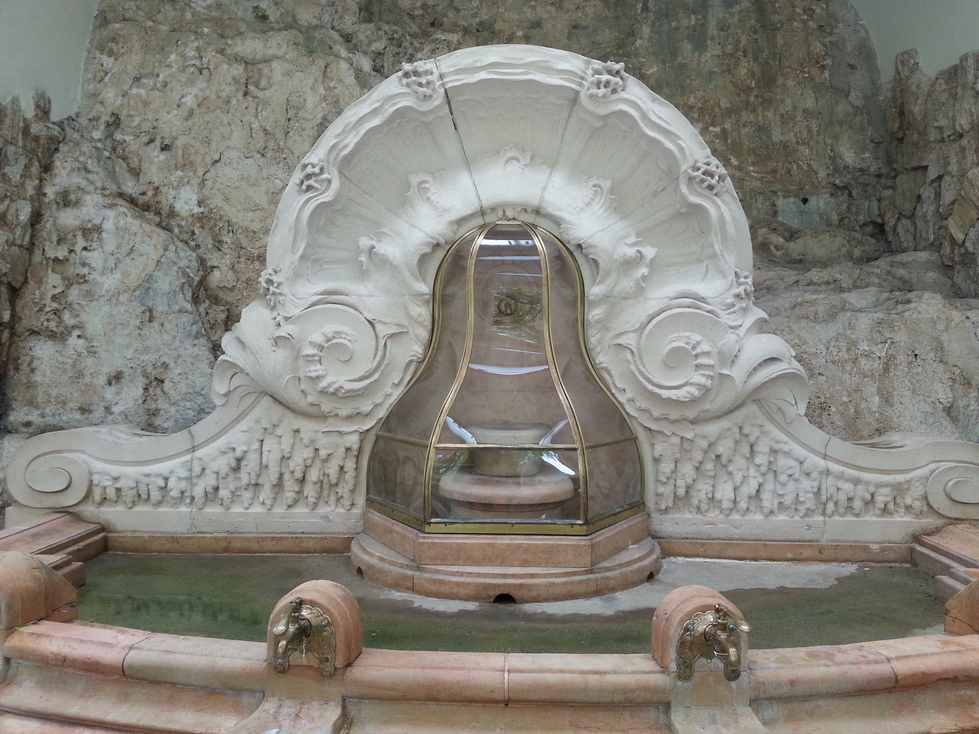
\includegraphics[height=0.3\textheight]{vichy-2}%
%  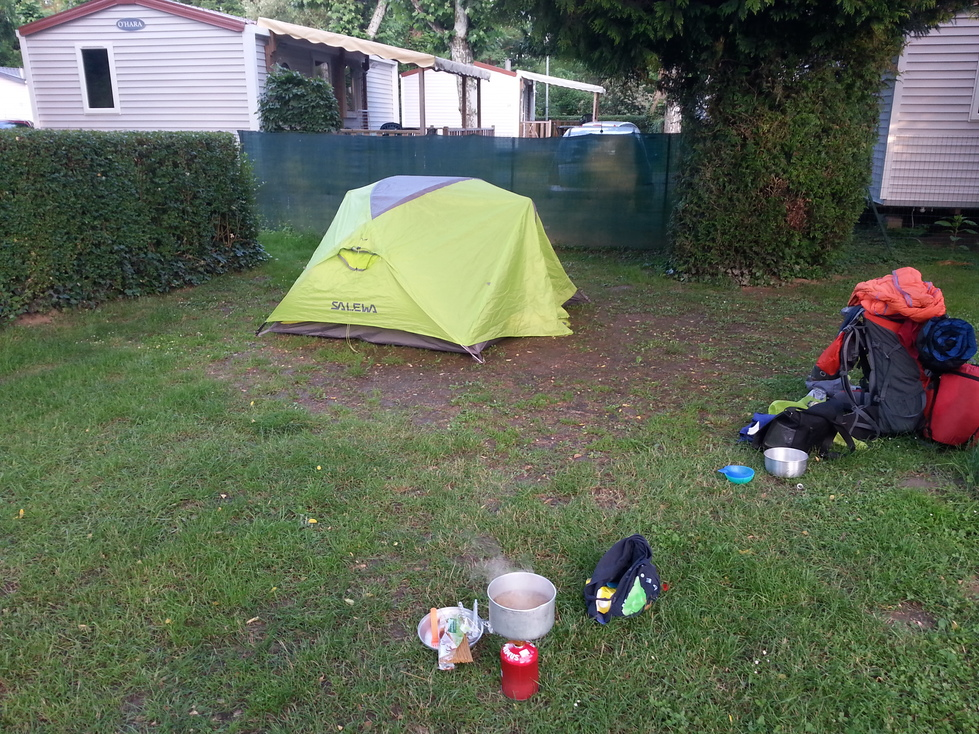
\includegraphics[height=0.3\textheight]{vichy-1}%
%  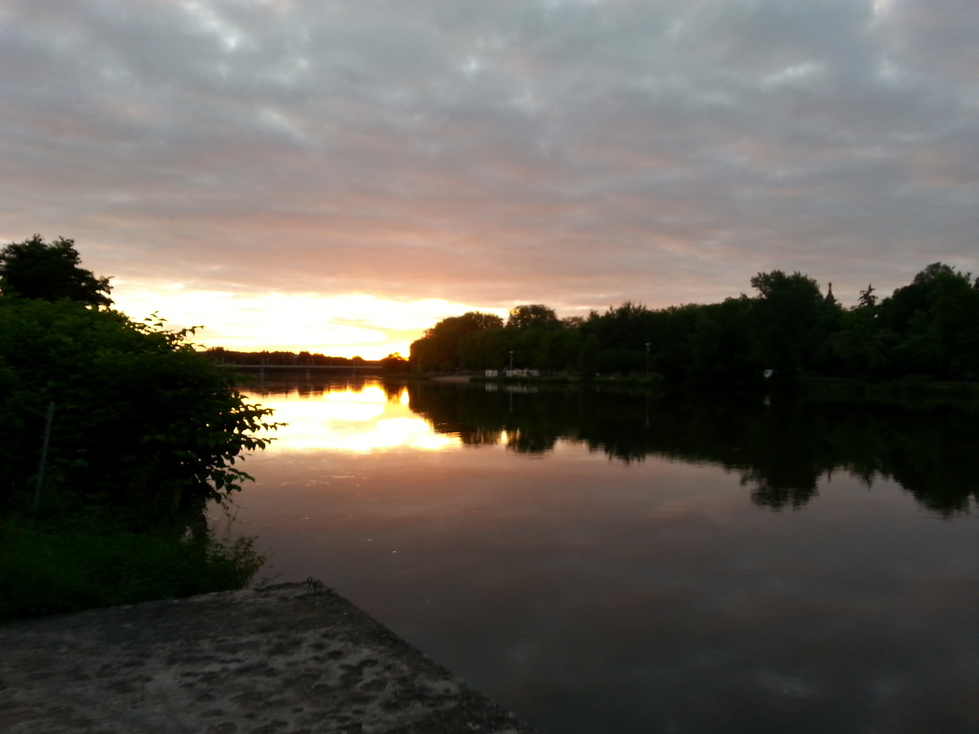
\includegraphics[height=0.3\textheight]{vichy-4}%
%  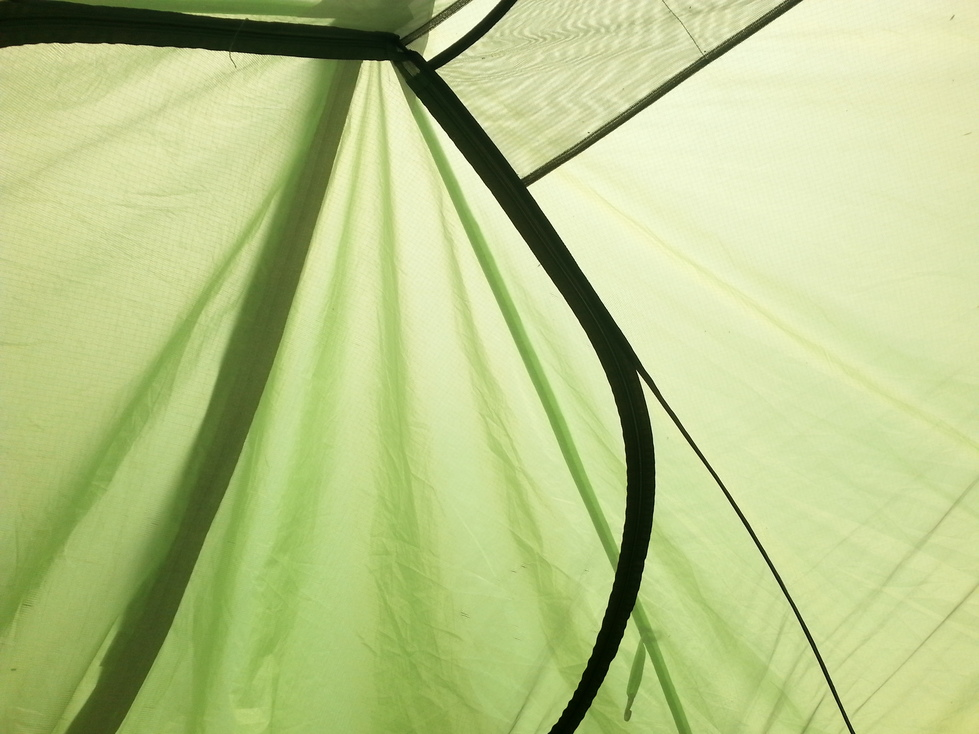
\includegraphics[height=0.3\textheight]{vichy-5}%

  \hil{Exploring the internal language of toposes} \\

  \emph{-- an invitation --}

  \bigskip

  \begin{columns}
    \small
    \begin{column}{0.35\textwidth}
      \centering
      \bignumber{1}
      
      \hil{Alternate universes}
      \medskip

    \end{column}
    \hspace*{0.5em}
    \begin{column}{0.25\textwidth}
      \centering
      \bignumber{2}
      
      \hil{Applications}
      \medskip

%      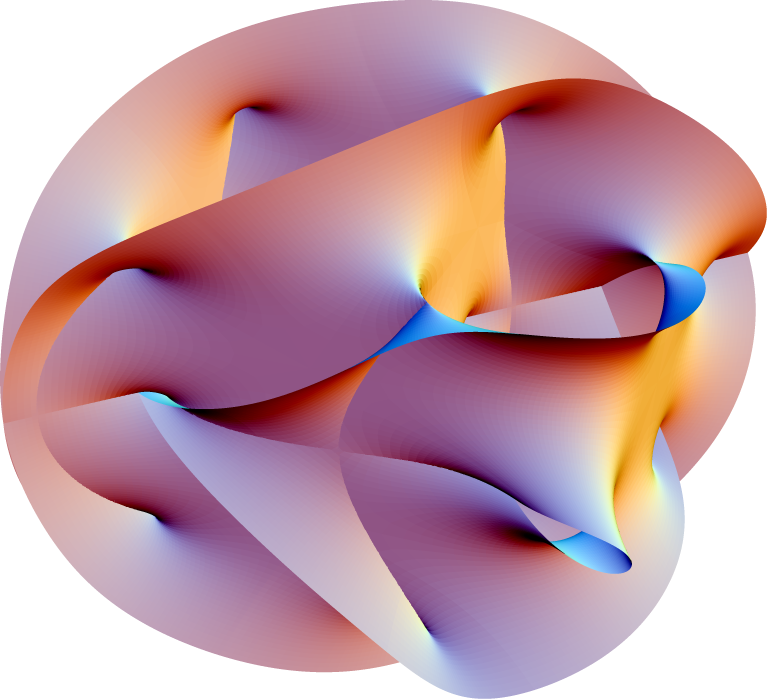
\includegraphics[height=5.5em]{calabi-yau}
    \end{column}
    \begin{column}{0.4\textwidth}
      \centering
      \bignumber{3}
      
      \hil{Vision for the future}
      \medskip

%      
\includegraphics[height=5.5em]{question-mark}
    \end{column}
  \end{columns}

  \scriptsize
  Ingo Blechschmidt (MPI Leipzig) \\
  Toposes in Como \\
  June 29th, 20s18
  \par
\end{frame}

\begin{frame}{Motivating testcases}
  Let $A$ be a ring (commutative, with unit, $1 = 0$ allowed). \\
  Assume that $A$ is reduced: If $x^n = 0$, then $x = 0$.

  \only<1-3>{\begin{columns}[t]
  \begin{column}[t]{0.50\textwidth}
    \centering

    \scalebox{0.8}{$\begin{pmatrix}
      \cdot & \cdot \\
      \cdot & \cdot \\
      \cdot & \cdot
      \end{pmatrix}$}
    \vspace*{-1em}

    \begin{varblock}{\textwidth}{A baby application}
      \justifying
      Let~$M$ be a surjective matrix over~$A$ with more rows than columns.
      Then~$1 = 0$ in~$A$.
    \end{varblock}

    \justifying
    \only<2>{\textbf{Proof.} \bad{Assume not.} Then there is~a \bad{maximal
    ideal} $\mmm$. The matrix is surjective over the field~$A/\mmm$. This is a
    contradiction to basic linear algebra.}

    \only<3>{\textbf{Proof.} \bad{Assume not.} Then there is~a \bad{prime
    ideal} $\ppp$. The matrix is surjective over the
    field~$\mathrm{Quot}(A/\ppp)$. This is a contradiction to basic linear
    algebra.}
  \end{column}

  \begin{column}[t]{0.5\textwidth}
    \centering

    \scalebox{0.8}{$\begin{pmatrix}
      \cdot & \cdot & \cdot & \cdot \\
      \cdot & \cdot & \cdot & \cdot \\
      \cdot & \cdot & \cdot & \cdot
    \end{pmatrix}$}
    \vspace*{-1em}

    \begin{varblock}{\textwidth}{A child application}
      \justifying
      Let~$M$ be an injective matrix over~$A$ with more columns than rows.
      Then~$1 = 0$ in~$A$.
    \end{varblock}
    
    \justifying
    \visible<2-3>{\textbf{Proof.} \bad{Assume not.} Then there is a \bad{minimal
    prime ideal} $\ppp$. The matrix is injective over the field~$A_\ppp = A[(A
    \setminus \ppp)^{-1}]$. This is a contradiction to basic linear algebra.}
    \end{column}
  \end{columns}}

  \pause
  \pause
  \pause

  \centering

  % XXX: 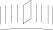
\includegraphics[height=3em]{generic-freeness}
  \vspace*{-1em}

  \begin{varblock}{0.9\textwidth}{Generic freeness$\phantom{p}$}
    \justifying
    Let~$B$ be an~$A$-algebra of finite type ($\cong A[X_1,\ldots,X_n]/\aaa$). \\
    Let~$M$ be a finitely generated~$B$-module ($\cong B^m/U$).

    If~$f = 0$ is the only element of~$A$ such that
    \begin{enumerate}
      \item $B[f^{-1}]$ and $M[f^{-1}]$ are free modules over $A[f^{-1}]$,
      \item $A[f^{-1}] \to B[f^{-1}]$ is of finite presentation and
      \item $M[f^{-1}]$ is finitely presented as a module over~$B[f^{-1}]$,
    \end{enumerate}
    then $1 = 0$ in~$A$.
  \end{varblock}
  \vspace*{-0.5em}

  \pause\raggedright
  \textbf{Proof.} See [Stacks Project, Tag 051Q].
\end{frame}

\begin{frame}{The internal language of a topos}
  For any topos~$\E$ and any formula~$\varphi$, we define the meaning of
  \vspace*{-0.5em}
  \[
    \text{``$\E \models \varphi$''} \quad
    \text{(``$\varphi$ holds in the internal universe of~$\E$'')}
  \]

  \vspace*{-1.0em}
  using (Shulman's extension of) the \hil{Kripke--Joyal semantics}.

  \vspace*{-1em}
  \begin{columns}
    \def\insertblocktitle{}
    \begin{column}{0.3\textwidth}\usebeamertemplate{block begin}
      \centering
      $\Set \models \varphi$ \\
      ``$\varphi$ holds in the \\ usual sense.''
      \usebeamertemplate{block end}\end{column}

    \begin{column}{0.3\textwidth}\usebeamertemplate{block begin}
      \centering
      $\Sh(X) \models \varphi$ \\
      ``$\varphi$ holds continuously.''
      \usebeamertemplate{block end}\end{column}

    \begin{column}{0.3\textwidth}\usebeamertemplate{block begin}
      \centering
      $\Eff \models \varphi$ \\
      ``$\varphi$ holds \\ computably.''
      \usebeamertemplate{block end}\end{column}
  \end{columns}
  \medskip

  Any topos supports \hil{mathematical reasoning}:

  \vspace*{-1.5em}
  \begin{hilblock}
    If~$\E \models \varphi$ and if~$\varphi$ entails~$\psi$
    \pointthis{<2>}{intuitionistically}{%
      no $\varphi \vee \neg\varphi$,\ \
      no $\neg\neg\varphi \Rightarrow \varphi$,\ \
      no axiom of choice},
    then~$\E \models \psi$.
  \end{hilblock}
\end{frame}

\begin{frame}{The internal language of~$\boldsymbol{\Sh(X)}$}
  \small
  Let~$X$ be a topological space. We recursively define
  \[ U \models \varphi \quad \text{(``$\varphi$ holds on~$U$'')} \]
  \mbox{for open subsets~$U \subseteq X$ and formulas~$\varphi$.
  Write~``$\Sh(X) \models \varphi$'' to mean~$X \models \varphi$.}
  \[ \renewcommand{\arraystretch}{1.25}\begin{array}{@{}l@{\ }c@{\ }l@{}}
  U \models f = g \? F &\Ll& f|_U = g|_U \in F(U) \\
  U \models \varphi \wedge \psi &\Ll&
  \text{$U \models \varphi$ and $U \models \psi$} \\
  U \models \varphi \vee \psi &\Ll&
  \hcancel{\text{$U \models \varphi$ or $U \models \psi$}}{0pt}{3pt}{0pt}{-2pt}\ \text{there exists a covering $U = \bigcup_i U_i$ s.\,th.} \\
  && \quad\quad\text{for all~$i$: $U_i \models \varphi$ or $U_i \models \psi$} \\
  U \models \varphi \Rightarrow \psi &\Ll&
  \text{for all open~$V \subseteq U$: } 
  \text{$V \models \varphi$ implies $V \models \psi$} \\
  U \models \forall f \? F\_ \varphi(f) &\Ll&
  \text{for all open $V \subseteq U$ and sections~$f_0 \in F(V)$: $V \models \varphi(f_0)$} \\
  U \models \forall F\_ \varphi(F) &\Ll&
  \text{for all open $V \subseteq U$ and sheaves~$F_0$ over~$V$: $V \models \varphi(F_0)$} \\
  U \models \exists f \? F\_ \varphi(f) &\Ll&
  \text{there exists a covering $U = \bigcup_i U_i$ s.\,th. for all~$i$:} \\
  && \quad\quad \text{there exists~$f_0 \in F(U_i)$ s.\,th. $U_i \models \varphi(f_0)$} \\
  U \models \exists F\_ \varphi(F) &\Ll&
  \text{there exists a covering $U = \bigcup_i U_i$ s.\,th. for all~$i$:} \\
  && \quad\quad \text{there exists a sheaf~$F_0$ on $U_i$ s.\,th. $U_i \models \varphi(F_0)$}
  \end{array} \]
\end{frame}

\begin{frame}{Internalizing parameter-dependence}
  \justifying
  Let~$X$ be a space. A continuous family~$(f_x)_{x \in X}$ of continuous
  functions (that is, a continuous function~$f : X \times \RR \to \RR$;
  $f_x(a) = f(x,a)$) induces an endomorphism of the sheaf~$\C$ of continuous
  functions:
  \[
    \bar f : \C \longrightarrow \C,\
    \text{on $U$:}\ s \longmapsto (x \mapsto f_x(s(x))).
  \]
  \begin{itemize}
    \item $\Sh(X) \models \speak{The set $\C$ is the set of (Dedekind) reals}$.
    \item $\Sh(X) \models \speak{The function $\bar f : \RR \to \RR$ is continuous}$.
    \item Iff $f_x(-1) < 0$ for all $x$, then $\Sh(X) \models \bar f(-1) < 0$.
    \item Iff $f_x(+1) > 0$ for all $x$, then $\Sh(X) \models \bar f(+1) > 0$.
    \item Iff all $f_x$ are increasing, then $\Sh(X) \models \speak{$\bar f$ is increasing}$.
    \item \ \\[-1.2em]\mbox{Iff there is an open cover~$X = \bigcup_i U_i$ such
    that for each~$i$ there is a} \mbox{continuous function~$s : U_i \to \RR$
    with~$f_x(s(x)) = 0$ for all~$x \in U_i$,} then $\Sh(X) \models \exists s
    \? \RR\_ \bar f(s) = 0$.
  \end{itemize}
\end{frame}

\begin{frame}{The little Zariski topos}
  Let~$A$ be a ring. Its \hil{little Zariski topos} is equivalently
  \begin{enumerate}
    \item the classifying topos of \hil{local localizations} of $A$,
    \item the classifying topos of \hil{prime filters} of $A$,
    \item the locale given by the frame of \hil{radical ideals} of $A$,
    \item the topos of sheaves over the poset $A$ with $f \preceq g$ iff $f \in \sqrt{(g)}$ and with $(f_i \to f)_i$ deemed covering iff $f \in \sqrt{(f_i)_i}$ or
    \item the topos of sheaves over $\Spec(A)$.
  \end{enumerate}
  Its associated topological space of points is the \hil{classical spectrum}
  \[ \{ \fff \subseteq A \,|\, \text{$\fff$ prime filter} \} + \text{Zariski topology}. \]
  It has \hil{enough points} if the Boolean Prime Ideal Theorem holds.

  \footnotesize
  Prime ideal:\, $0 \in \ppp$;\, $x \in \ppp \wedge y \in \ppp \Rightarrow x+y \in \ppp$;\, $1 \not\in \ppp$;\, $xy \in \ppp \Leftrightarrow x \in \ppp \vee y \in \ppp$

  Prime filter:\, $0 \not\in \fff$;\,\,
  $x+y \in \fff \Rightarrow x \in \fff \vee y \in \fff$;
  \hspace*{0.5pt}\,\,
  $1 \in \fff$;\,
  $xy \in \fff \Leftrightarrow x \in \fff \wedge y \in \fff$
\end{frame}

\begin{frame}{First steps in the little Zariski topos}
  Let~$A$ be a ring. Let~$\fff_0$ be the \hil{generic prime filter} of~$A$; it
  is a subobject of the constant sheaf~$\ull{A}$ of the little Zariski topos.

  \begin{itemize}
    \item The ring $A^\sim \defeq \ull{A}[\fff_0^{-1}]$ is the generic local
    localization of $A$.
    \item Given an~$A$-module~$M$, we have the~$A^\sim$-module $M^\sim \defeq
    \ull{M}[\fff_0^{-1}]$.
  \end{itemize}

  \only<1>{\begin{center}
    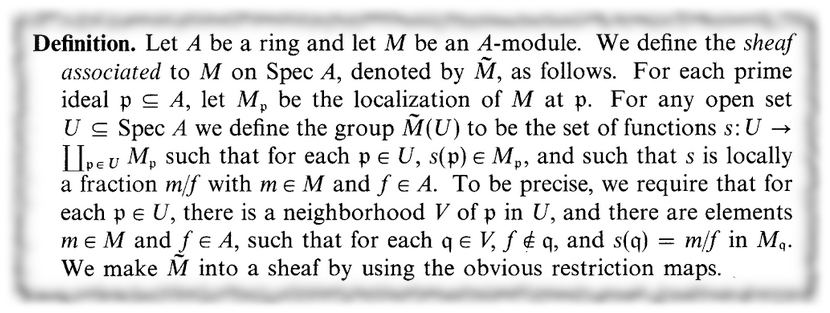
\includegraphics[width=0.9\textwidth]{hartshorne-tilde-construction} \\
    \footnotesize
    Robin Hartshorne. Algebraic Geometry. 1977.
  \end{center}}

  \pause

  \begin{columns}
    \begin{column}{0.5\textwidth}
      \begin{varblock}{\textwidth}{}
        \justifying
        Assuming the Boolean prime ideal theorem, a geometric sequent
        ``$\forall \ldots \forall\_ (\cdots \Longrightarrow \cdots\!\,)$'',
        where the two subformulas may not contain~``$\Rightarrow$'' and~``$\forall$'',
        holds for~$M^\sim$ iff it holds for all stalks~$M_\ppp$.
      \end{varblock}
    \end{column}

    \begin{column}{0.5\textwidth}
      \begin{varblock}{\textwidth}{}
        $M^\sim$ inherits any property of~$M$ which is \hil{localization-stable}.
      \end{varblock}

      \bigskip
      If $A$ is reduced ($x^n = 0 \Rightarrow x = 0$):

      \vspace*{-1em}
      \setbeamercolor{block body}{bg=red!30}
      \setbeamercolor{structure}{fg=purple}
      \begin{varblock}{\textwidth}{}
        $A^\sim$ is a \hil{field}
        (nonunits are zero).

        $A^\sim$ has \hil{$\boldsymbol{\neg\neg}$-stable equality}.

        \mbox{$A^\sim$ is \hil{anonymously Noetherian}.}\\[-1.2em]
      \end{varblock}
    \end{column}
  \end{columns}

  \visible<3>{\begin{tikzpicture}[overlay]
    \draw[fill=white, draw=white, opacity=0.95] (-1,0) rectangle (\paperwidth,7.4);
    \node[anchor=south west,inner sep=0] (image) at (0,0.8) {\vbox{
      \centering
      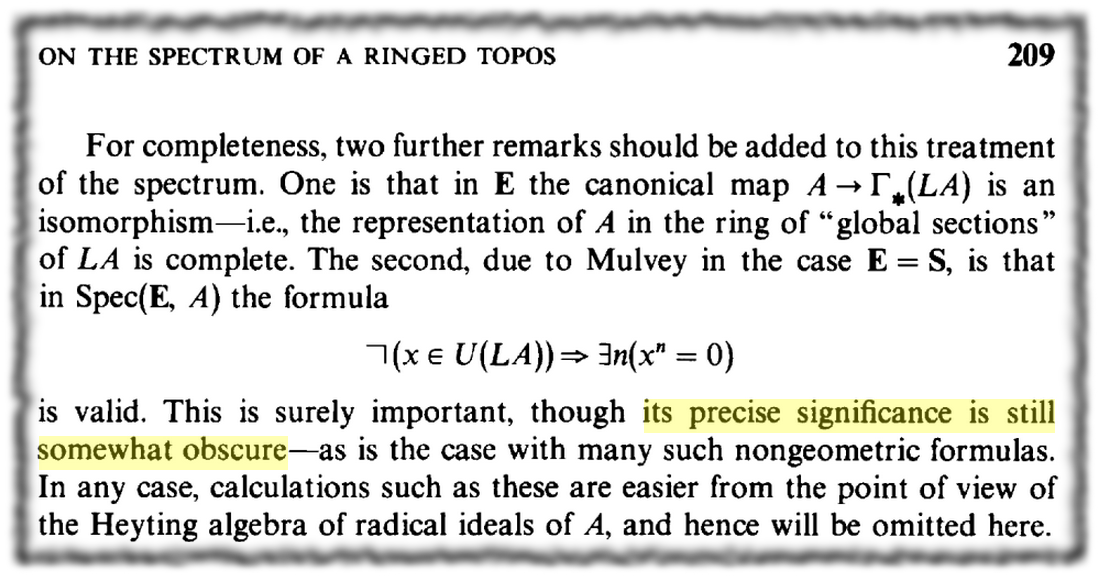
\includegraphics[width=0.9\textwidth]{tierney-on-the-spectrum-of-a-ringed-topos} \\
      \footnotesize
      Miles Tierney. On the spectrum of a ringed topos. 1976.
    }};
  \end{tikzpicture}}
\end{frame}

\begin{frame}{Revisiting the testcases}
  Let $A$ be a reduced ring.

  \only<1>{\begin{columns}[t]
    \begin{column}[t]{0.50\textwidth}
      \centering

      \scalebox{0.8}{$\begin{pmatrix}
        \cdot & \cdot \\
        \cdot & \cdot \\
        \cdot & \cdot
        \end{pmatrix}$}
      \vspace*{-1em}

      \begin{varblock}{\textwidth}{A baby application}
        \justifying
        Let~$M$ be a surjective matrix over~$A$ with more rows than columns.
        Then~$1 = 0$ in~$A$.
      \end{varblock}

      \justifying
      \textbf{Proof.} The matrix is surjective over the field~$A^\sim$. This is
      a contradiction to basic linear algebra. Hence $\Spec(A) \models \bot$,
      thus $1 = 0$ in $A$.
    \end{column}
    \begin{column}[t]{0.5\textwidth}
      \centering

      \scalebox{0.8}{$\begin{pmatrix}
        \cdot & \cdot & \cdot & \cdot \\
        \cdot & \cdot & \cdot & \cdot \\
        \cdot & \cdot & \cdot & \cdot
        \end{pmatrix}$}
      \vspace*{-1em}

      \begin{varblock}{\textwidth}{A child application}
        \justifying
        Let~$M$ be an injective matrix over~$A$ with more columns than rows.
        Then~$1 = 0$ in~$A$.
      \end{varblock}

      \justifying
      \textbf{Proof.} The matrix is injective over the field~$A^\sim$. This is
      a contradiction to basic linear algebra. Hence $\Spec(A) \models \bot$,
      thus $1 = 0$ in $A$.
    \end{column}
  \end{columns}}

  \pause

  \centering

  % XXX: 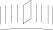
\includegraphics[height=3em]{generic-freeness}
  \vspace*{-1em}

  \begin{varblock}{\textwidth}{Generic freeness$\phantom{p}$}
    \justifying
    Let~$B$ be an~$A$-algebra of finite type ($\cong A[X_1,\ldots,X_n]/\aaa$). \\
    Let~$M$ be a finitely generated~$B$-module ($\cong B^m/U$).

    If~$f = 0$ is the only element of~$A$ such that
    \begin{enumerate}
      \item $B[f^{-1}]$ and $M[f^{-1}]$ are free modules over $A[f^{-1}]$, \\[-1.6em]
      \item $A[f^{-1}] \to B[f^{-1}]$ is of finite presentation and \\[-1.6em]
      \item $M[f^{-1}]$ is finitely presented as a module over~$B[f^{-1}]$,
    \end{enumerate}
    then $1 = 0$ in~$A$.
  \end{varblock}
  \vspace*{-0.5em}

  \pause\raggedright\bigskip
  \textbf{Proof.} In the little Zariski topos it's \hil{not not} the case that % \\[-1.4em]
  \begin{enumerate}
    \item $B^\sim$ and $M^\sim$ are free modules over $A^\sim$,
    \item $A^\sim \to B^\sim$ is of finite presentation and
    \item $M^\sim$ is finitely presented as a module over $B^\sim$
  \end{enumerate}
  by basic linear algebra over the field $A^\sim$. The claim is precisely the
  external translation of this fact.
\end{frame}

% Großer Zariskitopos
% Zusammenhang zum kleinen Topos
% Synthetische Quasikohärenz
% Klassifizierende Topoi

\begin{frame}{Understanding algebraic geometry}
  \vspace*{-1.5em}
  \begin{varblock}{0.9\textwidth}{}
    \justifying
    Understand \hil{notions of algebraic geometry} over a scheme~$X$ as
    \hil{notions of algebra} internal to~$\Sh(X)$.
  \end{varblock}

  \only<1>{
    \centering
    \rotatebox{90}{\tiny\scalebox{0.8}{Illustration: Carina Willbold}}\hspace{-0.05cm}%
    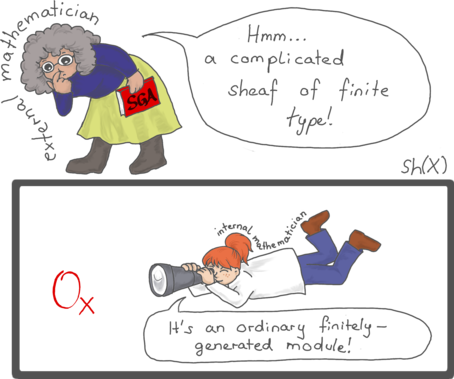
\includegraphics[width=0.7\textwidth]{external-internal-small}
    \par
  }

  \pause

  \small\centering
  \scalebox{0.83}{\begin{tabular}{ll}
    \toprule
    externally & internally to $\Sh(X)$ \\
    \midrule
    sheaf of sets & set \\
    %sheaf of rings & ring \\
    sheaf of modules & module \\
    sheaf of finite type & finitely generated module \\
    % finite locally free sheaf & finite free module \\
    % coherent sheaf & coherent module \\
    tensor product of sheaves & tensor product of modules \\
    % sheaf of Kähler differentials & module of Kähler differentials \\
    sheaf of rational functions & total quotient ring of~$\O_X$ \\
    dimension of $X$ & Krull dimension of~$\O_X$ \\
    spectrum of a sheaf of~$\O_X$-algebras & ordinary spectrum [with a twist] \\
    big Zariski topos of $X$ & big Zariski topos of the ring $\O_X$ [with a twist] \\
    higher direct images & sheaf cohomology \\
    \bottomrule
  \end{tabular}}

  \begin{columns}[c]
    \begin{column}{0.43\textwidth}
      \begin{exampleblock}{}
        \justifying
        Let~$0 \to M' \to M \to M'' \to 0$ be a short exact sequence of
        modules. If~$M'$ and~$M''$ are finitely generated, so is~$M$.
      \end{exampleblock}
    \end{column}

    \scalebox{3}{$\Rightarrow$}
    \hspace*{0.5em}

    \begin{column}{0.47\textwidth}
      \begin{exampleblock}{}
        \justifying
        Let $0 \to \F' \to \F \to \F'' \to 0$ be a short exact sequence
        of sheaves of~$\O_X$-modules. If~$\F'$ and~$\F''$ are of finite type,
        so is~$\F$.
      \end{exampleblock}
    \end{column}
  \end{columns}
\end{frame}

\begin{frame}{Synthetic algebraic geometry}
  Usual approach to algebraic geometry: \hil{layer schemes above ordinary set theory}
  using either
  \begin{itemize}
    \item locally ringed spaces
    \small
    \begin{multline*}
      \text{set of prime ideals of~$\ZZ[X,Y,Z]/(X^n+Y^n-Z^n)$} + {} \\
      \text{Zariski topology} + \text{structure sheaf}
    \end{multline*}
    \normalsize
    \item or Grothendieck's functor-of-points account, where a scheme is a
    functor~$\mathrm{Ring} \to \mathrm{Set}$.
    \small\[ A \longmapsto \{ (x,y,z) \in A^3 \,|\, x^n+y^n-z^n=0 \} \]
  \end{itemize}
  \bigskip

  \hil{Synthetic approach:} model schemes \hil{directly as sets} in a certain
  nonclassical set theory, the internal universe of the \mbox{\hil{big Zariski
  topos}} of a base scheme.
  \small
  \[ \{ (x,y,z) \? (\affl)^3 \,|\, x^n+y^n-z^n=0 \} \]
\end{frame}

\begin{frame}{The big Zariski topos}
  The \hil{big Zariski topos} $\Zar(S)$ of a scheme~$S$ is equivalently
  \begin{enumerate}
    \item the topos of sheaves over~$(\Aff/S)_{\mathrm{lofp}}$,
    \item the classifying topos of local rings over~$S$ or
    \item the classifying~$\Sh(S)$-topos of local~$\O_S$-algebras which are local
    over~$\O_S$.
  \end{enumerate}

  \begin{itemize}
    \item For an~$S$-scheme~$X$, its functor of points $\ull{X} =
    \Hom_S(\cdot,X)$ is an object of~$\Zar(S)$. It feels like \hil{the set of
    points} of~$X$.
    \item The ring $\affl$, given by $\affl(T) = \O_T(T)$,
    is a \hil{field} (nonzero implies invertible).
    \item \ \\[-1.2em]\mbox{$\ull{\mathbb{P}}^n = \llbracket \{ (x_0,\ldots,x_n) : (\affl)^{n+1} \,|\,
      x_0 \neq 0 \vee \cdots \vee x_n \neq 0 \}/(\affl)^\times \rrbracket$}
    \item $\ull{\Spec_S(\B)} = \llbracket \Hom_\affl(\B^\Zar,\affl) \rrbracket$
    \item $\ull{U} \hookrightarrow \ull{X}$ qc-open immersion iff
    \[ \Zar(S) \models \forall x\?\ull{X}\_ \bigvee_{n\geq0} \exists f_1,\ldots,f_n\?\affl\_ x \in \ull{U} \Leftrightarrow f_1 \neq 0 \vee \cdots \vee f_n \neq 0. \]
  \end{itemize}
\end{frame}

% XXX: Mehr Leute zitieren!
% XXX: Einordnung in Gesamtkontext (etwa SDG, Kock--Lawvere, Coquand & Co., ...)
% XXX: Folie zu klassifizierenden Topoi

\end{document}

\begin{frame}{The Kripke--Joyal semantics for the little Zariski topos}
  Recall~$A[f^{-1}] = \bigl\{ \frac{u}{f^n} \,|\, u \in A, n \in \NN \bigr\}$.

  \begin{itemize}
    \item $\Sh(\Spec(A)) \models \text{``For all~$x \in A^\sim$, \ldots''}$

          Meaning: For all~$f \in A$ and all~$x \in A[f^{-1}]$, \ldots
          \medskip

    \item $\Sh(\Spec(A)) \models \text{``There is~$x \in A^\sim$ such that \ldots''}$

          \mbox{Meaning: There is a partition of unity,~$1 = f_1 + \cdots + f_n \in A$,}
          such that for each~$i$, there exists~$x_i \in A[f_i^{-1}]$
          with~\ldots
          \medskip

    \item $\Sh(\Spec(A)) \models \text{``$\varphi$ implies $\psi$''}$

          Meaning: For all~$f \in A$, if~$\varphi$ on stage~$f$, then~$\psi$ on
          stage~$f$.
  \end{itemize}
\end{frame}

\section{Vision}

\begin{frame}{Vision for the future}
  \begin{columns}
    \small
    \begin{column}{0.35\textwidth}
      \centering
      \bigheart
      \par

      constructive algebra \\
      conceptual proofs \\
      proof assistants
    \end{column}

    \begin{column}{0.47\textwidth}
      \centering
      \bigheart
      \par

      constructive algebraic geometry \\
      synthetic algebraic geometry \\
      intersection theory \\
      derived categories
    \end{column}

    \begin{column}{0.25\textwidth}
      \centering
      \bigheart
      \par

      quasicoherence \\
      nongeometric mysteries \\
      further fields
    \end{column}
  \end{columns}

  \vfill

  \centering
  \href{https://www.oliviacaramello.com/Papers/Papers.htm}{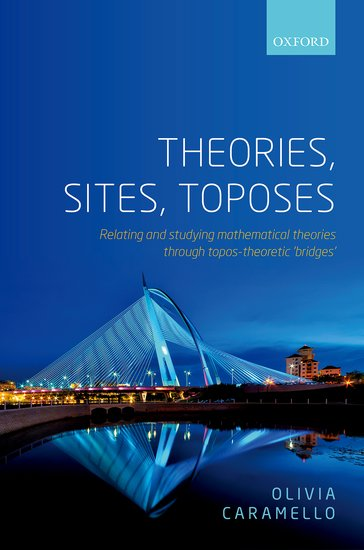
\includegraphics[height=0.45\textheight]{olivia-tst}}
  \href{http://math.andrej.com/2014/03/04/intuitionistic-mathematics-and-realizability-in-the-physical-world/}{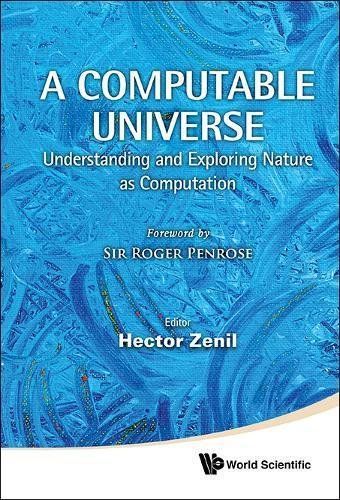
\includegraphics[height=0.45\textheight]{zenil-computable-universe}}
  \href{https://pizzaseminar.speicherleck.de/skript2/zariski-topos-klein.pdf}{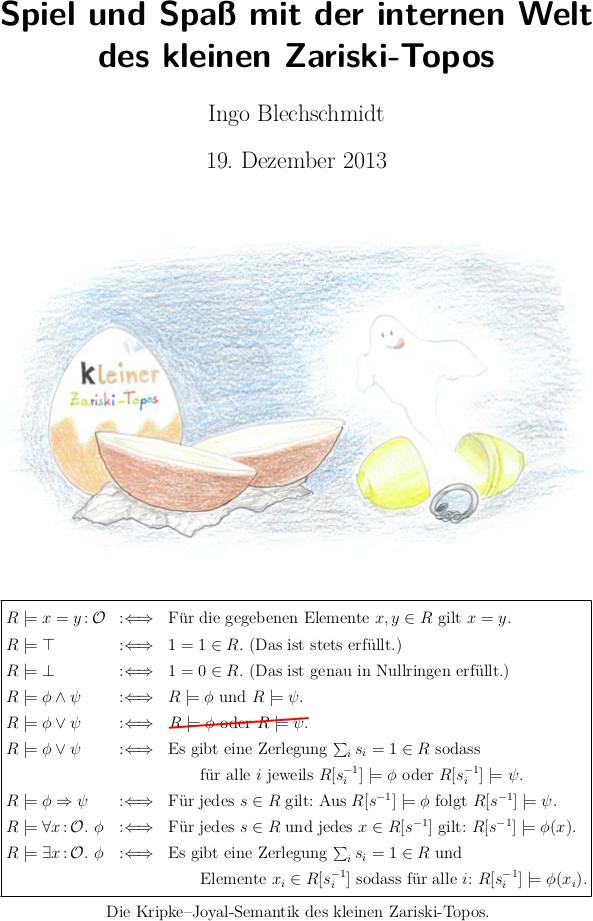
\includegraphics[height=0.45\textheight]{fun-with-the-zariski-topos}}
  \href{https://rawgit.com/iblech/internal-methods/master/notes.pdf}{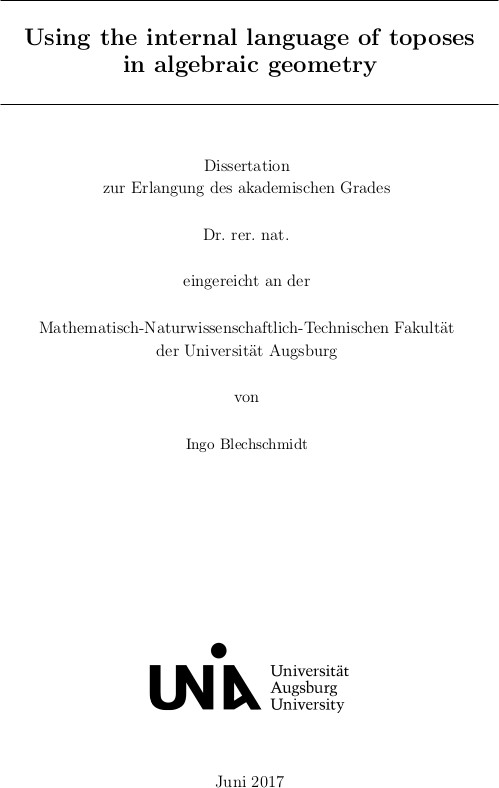
\includegraphics[height=0.45\textheight]{phd-cover}}
\end{frame}

\addtocounter{framenumber}{-1}

\end{document}
